% 2025 全国 1 卷 17：四棱锥 P-ABCD（PA⊥底面，AB⊥AD，BC∥AD）
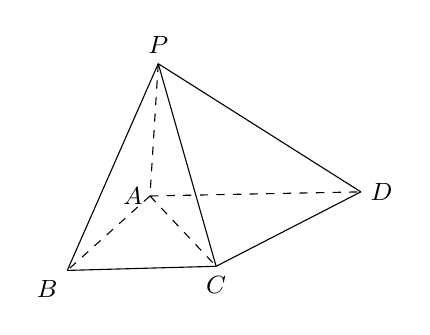
\begin{tikzpicture}[scale=1.05, font=\small]
  \coordinate (P) at (1.45,2.5);
  \coordinate (A) at (1.35,0.9);
  \coordinate (B) at (0.35,0);
  \coordinate (C) at (2.15,0.05);
  \coordinate (D) at (3.9,0.95);
  \draw (P) -- (B)  (P) -- (C)  (P) -- (D);
  \draw (B) -- (C) -- (D);
  \draw[dashed] (P) -- (A);
  \draw[dashed] (A) -- (B)  (A) -- (D)  (A) -- (C);
  \node[above] at (P) {$P$};
  \node[left, inner sep=2.5pt] at (A) {$A$};
  \node[below left] at (B) {$B$};
  \node[below] at (C) {$C$};
  \node[right] at (D) {$D$};
\end{tikzpicture}
